\documentclass[11pt,a4paper]{article}

% ------------------------------------------------------------------ packages
\usepackage[margin=2.1cm]{geometry}
\usepackage[T1]{fontenc}
\usepackage{lmodern}
\usepackage{microtype}
\usepackage{graphicx}
\usepackage{booktabs}
\usepackage{tabularx}
\usepackage{array}
\usepackage{amsmath}
\usepackage{enumitem}
\usepackage{xcolor}
\usepackage[most]{tcolorbox}
\usepackage{tikz}
\usetikzlibrary{arrows.meta,positioning,shapes.geometric}
\usepackage{caption}
\usepackage{float}
\usepackage{hyperref}
\hypersetup{colorlinks=true,linkcolor=blue!50!black,urlcolor=blue!60!black,citecolor=blue!50!black}

\graphicspath{{figures/}{../results/figures/}}
\setlist{itemsep=2pt,topsep=3pt}
\captionsetup{font=small,labelfont=bf}
\renewcommand{\arraystretch}{1.15}

\newtcolorbox{keybox}[1]{colback=blue!4,colframe=blue!45!black,fonttitle=\bfseries,title=#1,boxrule=0.6pt,arc=2pt}

% ================================================================== document
\begin{document}

% ------------------------------------------------------------------ cover
\begin{titlepage}
\centering
\vspace*{1.2cm}
{\large\scshape Market Microstructure\par}
{\large Term Project Report\par}
\vspace{2.2cm}
\rule{\textwidth}{0.8pt}\par\vspace{0.5cm}
{\LARGE\bfseries The Role of Dealers:\par}
\vspace{0.25cm}
{\Large Do Dealer-Like Liquidity Providers Absorb\\ Temporary Liquidity Shocks?\par}
\vspace{0.4cm}
\rule{\textwidth}{0.8pt}\par
\vspace{2.2cm}

{\large\bfseries Team Members\par}
\vspace{0.4cm}
\begin{tabular}{ll}
\toprule
\textbf{Name} & \textbf{Roll Number} \\
\midrule
Member 1 Name & \hspace{3cm} \\
Member 2 Name & \\
Member 3 Name & \\
Member 4 Name & \\
\bottomrule
\end{tabular}

\vspace{2cm}
{\large Course Instructor: \underline{\hspace{6cm}}\par}
\vspace{0.4cm}
{\large Department / Institute: \underline{\hspace{6cm}}\par}
\vfill
{\normalsize Code, data pipeline and results: \url{https://github.com/sharanyabaidya/Market_Micro_Project}\par}
\vspace{0.3cm}
{\large October 2026\par}
\end{titlepage}

% ------------------------------------------------------------------ contents
\tableofcontents
\vspace{0.6cm}

\begin{keybox}{Project material (click to open)}
\begin{tabular}{@{}l p{11.8cm}@{}}
Repository & \url{https://github.com/sharanyabaidya/Market_Micro_Project}\\
Full results report & \href{https://github.com/sharanyabaidya/Market_Micro_Project/blob/main/REPORT.md}{REPORT.md}\\
Audit of every test & \href{https://github.com/sharanyabaidya/Market_Micro_Project/blob/main/VALIDATION_LOG.md}{VALIDATION\_LOG.md}\\
Executed notebook & \href{https://github.com/sharanyabaidya/Market_Micro_Project/blob/main/notebooks/analysis.ipynb}{notebooks/analysis.ipynb}\\
Result tables / figures & \href{https://github.com/sharanyabaidya/Market_Micro_Project/tree/main/results/tables}{results/tables} \;/\; \href{https://github.com/sharanyabaidya/Market_Micro_Project/tree/main/results/figures}{results/figures}\\
Source code & \href{https://github.com/sharanyabaidya/Market_Micro_Project/tree/main/src/mm}{src/mm} \;(run with \href{https://github.com/sharanyabaidya/Market_Micro_Project/blob/main/scripts/run_all.py}{scripts/run\_all.py})\\
Original proposal & \href{https://github.com/sharanyabaidya/Market_Micro_Project/blob/main/Market_Micro_Project_Proposal.pdf}{Market\_Micro\_Project\_Proposal.pdf}\\
\end{tabular}
\end{keybox}

\vspace{0.4cm}
\noindent\textbf{One-paragraph summary.}
Dealers are supposed to stand ready to trade when others want to buy or sell urgently, absorbing temporary
order imbalances and earning a spread for the risk. Modern stock markets have no designated dealers; liquidity
comes from anyone posting limit orders. We ask whether these \emph{dealer-like} liquidity providers behave as
the classic dealer models predict when order flow suddenly becomes extremely one-sided. Using two public
limit order book datasets (FI-2010, Helsinki; LOBSTER, NASDAQ) we find that liquidity is drained on the side
being hit and refills quickly, but providers do \emph{not} lean against the flow, prices do \emph{not} bounce
back, and those who absorb the shock lose money to better-informed traders.

\newpage

% ================================================================== 1 PROBLEM
\section{Problem Statement: The Role of Dealers}
\label{sec:problem}

\subsection{What a dealer does}
A trader who wants to sell \emph{now} needs someone willing to buy \emph{now}. In a dealer market this
counter-party is the dealer: a market maker who quotes a \textbf{bid} (the price at which it buys) and an
\textbf{ask} (the price at which it sells) and trades with anyone who arrives. The dealer therefore provides
\emph{immediacy}. In exchange it earns the \textbf{bid--ask spread}, but it also bears two risks:
\begin{itemize}
  \item \textbf{Inventory risk}: after buying from many sellers the dealer holds an unwanted position whose
        value can fall.
  \item \textbf{Adverse selection}: some of the people it trades with know more than it does; trading with
        them loses money on average.
\end{itemize}
How dealers manage these risks determines how prices and liquidity respond when many traders want to trade
in the same direction at the same time --- a \emph{temporary liquidity shock}.

\subsection{What the four suggested papers say}
\begin{description}[leftmargin=0pt]
\item[Amihud \& Mendelson (1980) --- inventory.] A single dealer sets its quotes as a function of its inventory.
  After buying too much, it \emph{lowers both bid and ask} to attract buyers and discourage further sellers;
  the spread is wider when inventory is far from its target. \emph{Prediction:} order imbalances move prices
  only temporarily, and prices drift back as the dealer unloads its position.
\item[Ho \& Stoll (1983) --- competing dealers.] With several dealers, each shades its quotes according to its
  own inventory, and the best quote in the market comes from the dealer most eager to trade.
  \emph{Prediction:} more competition gives narrower spreads; quotes respond to trades in an inventory-driven way.
\item[Biais \& Weill (2009) --- liquidity shocks in an order book.] Traders hit by a shock want to trade at once,
  but others can only return to the market gradually. The book becomes one-sided and thin, then refills over
  time. \emph{Prediction:} after a shock, liquidity is drained and recovers gradually; price pressure fades
  as the book refills.
\item[Biais, Declerck \& Moinas (2016) --- who supplies liquidity.] Liquidity is supplied by different types of
  traders (fast proprietary traders, slower institutions, designated market makers). Fast traders supply
  much of the liquidity in normal times but provide less when order flow is one-sided.
  \emph{Prediction:} the composition of liquidity suppliers changes under stress, and those who keep
  supplying bear adverse-selection costs.
\end{description}

\subsection{From dealer markets to limit order books}
The two dealer models (Amihud--Mendelson, Ho--Stoll) were written for markets with identifiable dealers.
Today's equity markets are \textbf{limit order books}: anyone can post a limit order and thereby act like a
dealer for a moment. There is no observable ``dealer inventory'' and no list of dealers. The relevant question
therefore becomes: \emph{does the collective behaviour of passive liquidity providers look like the behaviour
the dealer papers predict?} We call this \textbf{dealer-like liquidity provision}.

\subsection{Research question and hypotheses}
\begin{keybox}{Research question}
Do dealer-like liquidity providers absorb temporary liquidity shocks, and does their provision help prices
and market liquidity recover?
\end{keybox}

\noindent The mechanism we test is
\emph{liquidity shock $\rightarrow$ liquidity provision $\rightarrow$ shock absorption $\rightarrow$ price
and liquidity stabilisation}, broken into four hypotheses:

\begin{center}
\begin{tabularx}{\linewidth}{@{}l X l@{}}
\toprule
& \textbf{Hypothesis} & \textbf{Main paper} \\
\midrule
H1 & Shocks are associated with wider spreads, lower depth and stronger order imbalance. & Biais--Weill \\
H2 & After a shock, liquidity providers act \emph{against} the prevailing pressure (contrarian provision). & Amihud--Mendelson, Ho--Stoll \\
H3 & Stronger provision is followed by faster recovery of prices and liquidity. & Biais--Weill \\
H4 & Providing liquidity during a shock exposes providers to adverse-selection costs. & Biais--Declerck--Moinas \\
\bottomrule
\end{tabularx}
\end{center}

\noindent\textbf{Why it matters.} If providers absorb shocks and prices revert, temporary imbalances are
harmless and self-correcting. If instead providers step back and prices stay moved, shocks have lasting
effects and the ``dealer'' function is weaker than textbook models assume --- relevant for market design,
market-maker obligations and the regulation of fast trading.

\newpage
% ================================================================== 2 DATA
\section{Data Sources}
\label{sec:data}

\begin{center}
\begin{tabularx}{\linewidth}{@{}l X X@{}}
\toprule
& \textbf{FI-2010} \cite{ntakaris2018} & \textbf{LOBSTER sample files} \cite{lobster} \\
\midrule
Market & Nasdaq Nordic Helsinki & NASDAQ (US) \\
Stocks & Kesko, Outokumpu, Sampo, Rautaruukki, W\"artsil\"a & Apple, Amazon, Google, Intel, Microsoft \\
Period & 10 trading days, June 2010 & 1 trading day, 21 June 2012 \\
Content & 10 price levels of the book, one snapshot every 10 order-book events (394{,}337 snapshots) & 10 price levels \emph{plus} every message: new orders, cancellations, trades, order IDs, trade direction \\
Strength & Many days $\Rightarrow$ 50 stock-days & Trades and order IDs $\Rightarrow$ who trades with whom \\
Weakness & No timestamps, no trades & Only one day \\
Access & Public benchmark (mirror in the DeepLOB repository \cite{deeplob}) & Free samples (\url{https://lobsterdata.com}) \\
\bottomrule
\end{tabularx}
\end{center}

\noindent Raw data are \emph{not} stored in the repository; \href{https://github.com/sharanyabaidya/Market_Micro_Project/blob/main/scripts/download_data.sh}{scripts/download\_data.sh}
downloads them. Two data-cleaning steps were essential:
\begin{enumerate}
  \item FI-2010 files concatenate all stocks and days into one long series. We split them exactly into
        50 stock-days by detecting the overnight rebuild of the book (no order survives from one snapshot to
        the next). Without this step, event windows mix different stocks.
  \item In LOBSTER, the direction field of \emph{hidden} executions is unreliable (in Intel and Microsoft it
        agrees with the actual trade side only $\sim$15\% of the time). Hidden trades are therefore signed by
        comparing the price with the mid-price; visible trades are signed exactly.
\end{enumerate}

% ================================================================== 3 METHOD
\section{Methodology Pipeline}
\label{sec:method}

\begin{figure}[H]
\centering
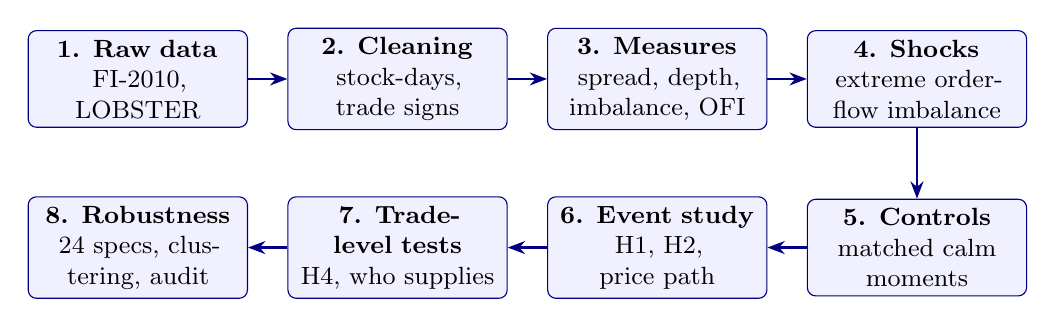
\begin{tikzpicture}[node distance=0.45cm and 0.5cm,
  box/.style={rectangle,rounded corners=3pt,draw=blue!50!black,fill=blue!6,align=center,
              minimum height=1.05cm,text width=2.55cm,font=\small},
  arr/.style={-{Stealth[length=2.2mm]},thick,blue!50!black}]
\node[box] (a) {\textbf{1. Raw data}\\FI-2010, LOBSTER};
\node[box,right=of a] (b) {\textbf{2. Cleaning}\\stock-days, trade signs};
\node[box,right=of b] (c) {\textbf{3. Measures}\\spread, depth, imbalance, OFI};
\node[box,right=of c] (d) {\textbf{4. Shocks}\\extreme order-flow imbalance};
\node[box,below=0.9cm of d] (e) {\textbf{5. Controls}\\matched calm moments};
\node[box,left=of e] (f) {\textbf{6. Event study}\\H1, H2, price path};
\node[box,left=of f] (g) {\textbf{7. Trade-level tests}\\H4, who supplies};
\node[box,left=of g] (h) {\textbf{8. Robustness}\\24 specs, clustering, audit};
\draw[arr] (a)--(b); \draw[arr] (b)--(c); \draw[arr] (c)--(d); \draw[arr] (d)--(e);
\draw[arr] (e)--(f); \draw[arr] (f)--(g); \draw[arr] (g)--(h);
\end{tikzpicture}
\caption{Analysis pipeline (code in the folder \texttt{src/mm} of the repository).}
\end{figure}

\paragraph{Liquidity measures.} With best ask $A_t$ and best bid $B_t$:
mid-price $M_t=(A_t+B_t)/2$, spread $S_t=A_t-B_t$, relative spread $S_t/M_t$ (in basis points),
depth = shares resting on the first 1, 3 or 10 levels, and book imbalance
$(D^{bid}-D^{ask})/(D^{bid}+D^{ask})$.

\paragraph{Order-flow imbalance (OFI).} The proposal's imbalance formula uses resting depth, which measures
the \emph{stock} of orders, not the \emph{flow} of buying or selling pressure. We use the order-flow
imbalance of Cont, Kukanov \& Stoikov \cite{cont2014}, which adds up, between two snapshots, new bids and
removed asks (buying pressure) minus new asks and removed bids (selling pressure) at the best quotes.

\paragraph{Shock definition.} A \emph{sell (buy) shock} occurs when OFI summed over 5 steps (50 book events)
falls in the bottom (top) 1\% of that stock's distribution. Shocks are at least 100 steps apart and never cross
a day or stock boundary. This gives \textbf{1{,}269 shocks} in FI-2010 and \textbf{657} in LOBSTER.

\paragraph{Matched controls (the key design choice).} Book variables drift back to normal by themselves, so a
plain before/after comparison would wrongly look like ``recovery''. Each shock is therefore compared with
5 calm moments from the same stock and day that have a similar order book:
(i) matched \emph{before} the shock, to measure what the shock did; and
(ii) matched on the \emph{same depleted book after} the shock, to tell genuine contrarian provision apart
from normal refilling. All effects are \emph{shock minus control} (difference-in-differences).

\paragraph{Time windows.} Shock $[-5,0]$, provision $(0,10]$, recovery $(10,100]$, long run up to 300 steps
(one step = 10 book events; in LOBSTER 100 steps $\approx$ 0.5--2.5 minutes).

\paragraph{Statistics.} Events from the same stock-day are not independent, so standard errors are clustered
by stock-day (FI-2010) or by stock $\times$ 30 minutes (LOBSTER); 95\% confidence intervals are reported and
$p$-values are corrected for multiple testing (Holm).

% ================================================================== 4 EXPERIMENTS
\section{Experiments Performed}
\label{sec:experiments}

\begin{center}
\begin{tabularx}{\linewidth}{@{}l X l@{}}
\toprule
\# & \textbf{Experiment} & \textbf{Answers} \\
\midrule
E1 & Event study of spread, depth and imbalance around shocks vs.\ matched controls & H1 \\
E2 & Contrarian order flow, refilling of the hit side and price-improving quotes after the shock, vs.\ controls with the same depleted book & H2 \\
E3 & Regression of recovery (price reversal, spread, depth) on the strength of provision & H3 \\
E4 & Trade level (LOBSTER): price impact and realised spread of trades during shocks vs.\ normal trades & H4 \\
E5 & Price path after shocks and after ordinary trades, up to 10 minutes in clock time & reversal? \\
E6 & Who supplies liquidity: age of the resting orders that get executed, normal vs.\ shock & BDM \\
E7 & Dealer-theory proxies: inventory, spread vs.\ imbalance, competition, Huang--Stoll decomposition & AM, HS \\
E8 & Robustness: 24 specifications per dataset, alternative clustering, placebo tests, full audit & all \\
\bottomrule
\end{tabularx}
\end{center}

% ================================================================== 5 RESULTS
\section{Results}
\label{sec:results}

\begin{table}[H]
\centering\small
\caption{Main estimates (shock minus matched control; 95\% confidence intervals in brackets).}
\label{tab:main}
\begin{tabularx}{\linewidth}{@{}l X X@{}}
\toprule
\textbf{Measure} & \textbf{FI-2010 (1{,}269 shocks)} & \textbf{LOBSTER (657 shocks)} \\
\midrule
\multicolumn{3}{@{}l}{\emph{H1 -- liquidity deterioration}}\\
Best-level depth on hit side ($\times$ mean) & $-0.56$ [$-0.66$, $-0.47$] & $0.00$ [$-0.24$, $0.23$] \\
Book imbalance toward the pressure & $+0.15$ [$0.12$, $0.19$] & $+0.12$ [$0.07$, $0.17$] \\
Relative spread (bps) & $+0.39$ [$-0.13$, $0.92$] n.s. & $+0.75$ [$0.44$, $1.07$] \\
\midrule
\multicolumn{3}{@{}l}{\emph{H2 -- contrarian provision (vs.\ same depleted book)}}\\
Order flow against the shock, next 10 steps & $-0.56$ [$-0.87$, $-0.24$] & $-1.00$ [$-1.45$, $-0.55$] \\
Refill of the hit side & $+0.02$ n.s. & $+0.05$ n.s. \\
Price-improving quotes on the hit side & $-0.07$ (n.s. after correction) & $-0.21$ [$-0.34$, $-0.07$] \\
\midrule
\multicolumn{3}{@{}l}{\emph{Prices after the shock}}\\
Further drift in shock direction, 100 steps (bps) & $+5.0$ [$3.3$, $6.6$] & $+1.3$ [$0.8$, $1.7$] \\
\midrule
\multicolumn{3}{@{}l}{\emph{H4 -- adverse selection, shock trades vs.\ normal trades (LOBSTER)}}\\
Price impact after 5 s (bps) & -- & $+1.23$ [$0.80$, $1.66$] \\
Realised spread after 5 s (bps) & -- & $-1.14$ [$-1.51$, $-0.78$] \\
Effective half-spread (bps) & -- & $+0.09$ [$-0.03$, $0.21$] n.s. \\
\bottomrule
\end{tabularx}
\end{table}

\noindent\textbf{H3} (provision $\rightarrow$ faster recovery): no provision measure predicts price or
liquidity recovery after correcting for multiple tests; some support appears only for mild shocks in
FI-2010.

\begin{figure}[H]
\centering
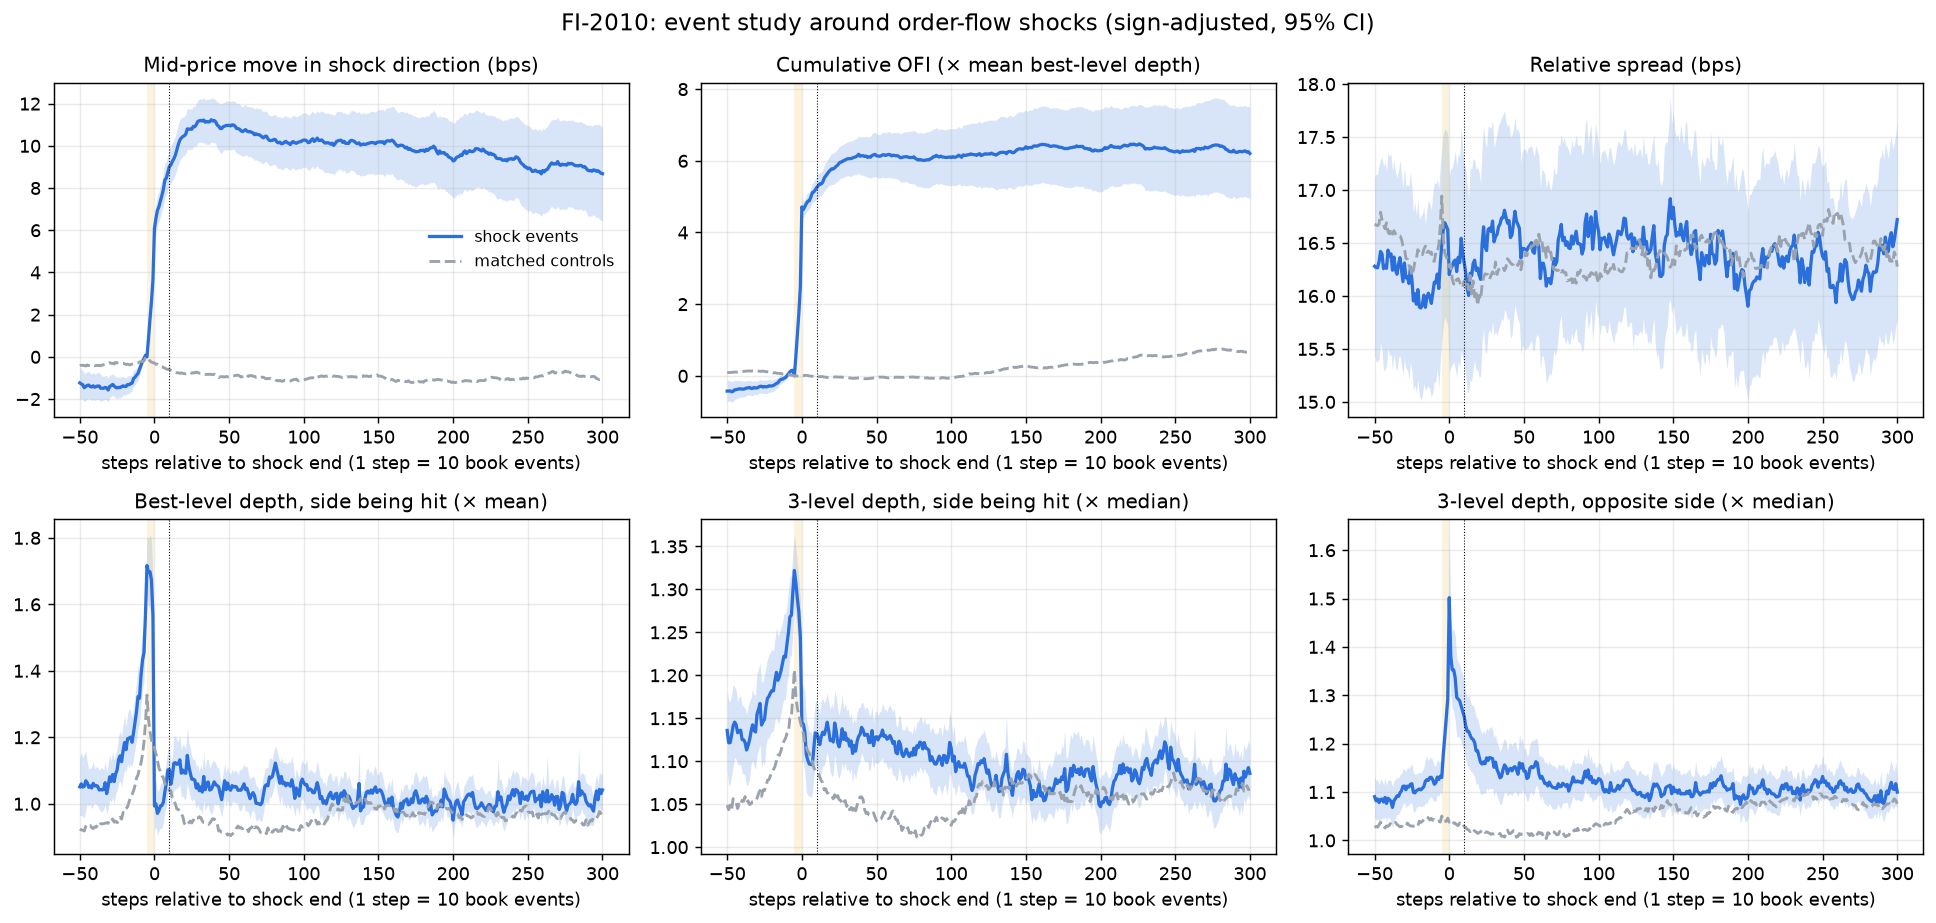
\includegraphics[width=\linewidth]{fig1_event_study_FI-2010.png}
\caption{FI-2010 event study (blue: shocks; grey: matched controls; shaded: shock window). The price keeps
moving in the shock direction, order flow keeps pushing, and best-level depth on the hit side collapses and
then refills.}
\end{figure}

\begin{figure}[H]
\centering
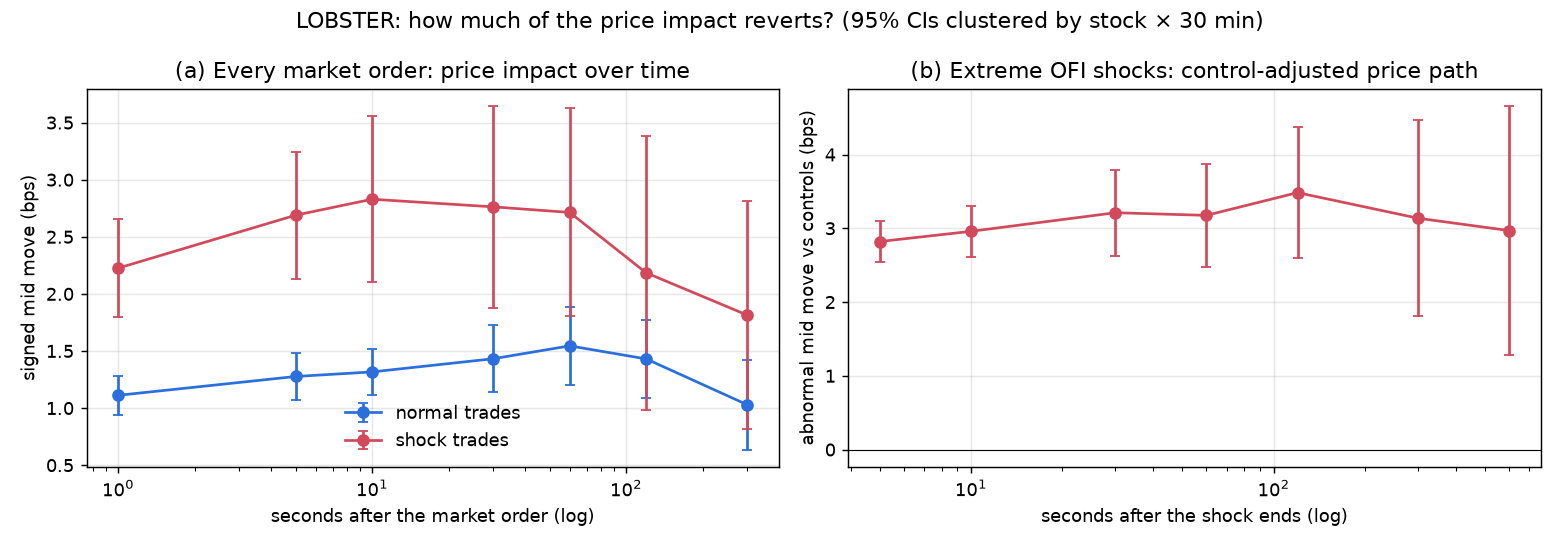
\includegraphics[width=0.92\linewidth]{fig2_price_response_LOBSTER.png}
\caption{(a) After an ordinary trade about a third of the price impact reverts within 5 minutes.
(b) After an extreme order-flow shock, about 85\% of the peak price move is still present after 10 minutes.}
\end{figure}

\begin{figure}[H]
\centering
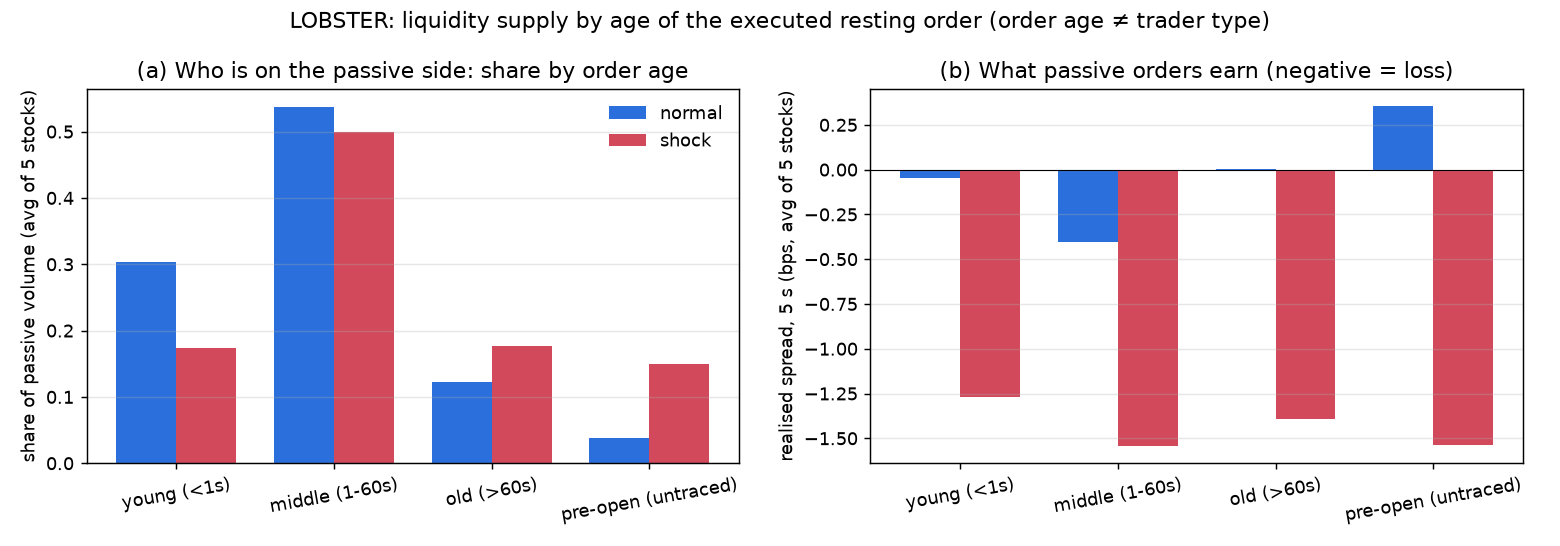
\includegraphics[width=0.92\linewidth]{fig3_liquidity_supply_by_order_age_LOBSTER.png}
\caption{Who is on the passive side of trades. During shocks, very young (re-priced, fast) orders supply a
smaller share of liquidity and older resting orders a larger share; all groups lose money on shock trades.}
\end{figure}

% ================================================================== 6 FINDINGS
\section{Key Findings}
\label{sec:findings}

\begin{keybox}{Five key findings}
\begin{enumerate}[leftmargin=*]
\item \textbf{Shocks drain liquidity where the pressure hits.} Best-level depth on the side being hit falls by
  about 56\% of its normal level (FI-2010, all five stocks) and the book tilts toward the pressure; spreads
  widen in LOBSTER (+0.75 bps, about 18\%) and recover within seconds. \hfill \emph{H1 supported (spread: mixed)}
\item \textbf{Providers do not lean against the flow.} Compared with the same thin book in calm times, order flow
  keeps pushing in the shock direction, the hit side refills no faster, and there are fewer price-improving
  quotes. Same sign in all 24 specifications per dataset. \hfill \emph{H2 contradicted}
\item \textbf{Prices after shocks largely stay moved.} Ordinary trades show partial reversal (about one third
  within 5 minutes), but after extreme shocks about 85\% of the price move persists for 10 minutes --- unlike
  the temporary price pressure predicted by inventory models. \hfill \emph{H3 mixed}
\item \textbf{Absorbing a shock is costly.} Liquidity providers on the other side of shock trades lose about
  1.1 bps more per trade than in normal times and are not compensated by wider spreads. \hfill \emph{H4 supported}
\item \textbf{The suppliers change under stress.} The share of passive volume coming from very young orders
  (under 1 second old) falls from 30\% to 17\% during shocks, while older and pre-open orders absorb more ---
  consistent with Biais--Declerck--Moinas. Order age is a proxy, not trader identity.
\end{enumerate}
\end{keybox}

\noindent\textbf{Overall.} Liquidity in these limit order books recovers quickly (as in Biais--Weill), but the
classic dealer role --- leaning against order imbalances and earning a reward when prices revert --- is weak.
Shocks look more like information arriving than like temporary inventory pressure.

% ================================================================== 7 ASSUMPTIONS
\section{Assumptions, Limitations and Future Scope}
\label{sec:limits}

\subsection{Major assumptions}
\begin{enumerate}
\item \textbf{Dealer-like = passive side of trades.} All limit-order providers together are treated as
      ``the dealer''; their combined position change is minus the signed market-order flow.
\item \textbf{Shocks are extreme order-flow imbalance.} A 1\%-tail OFI event over 50 book events is taken to be
      a liquidity shock; shocks are defined from market data, not from news.
\item \textbf{Matched calm moments are valid counterfactuals.} Controls from the same stock and day with a
      similar book represent what would have happened without the shock.
\item \textbf{Event time is a valid clock.} One step = 10 book events (FI-2010 has no timestamps).
\item \textbf{Trade signs.} Visible executions are signed exactly; hidden executions by price vs.\ mid-price,
      dropping those exactly at the mid.
\item \textbf{Order age measures speed.} Time since an order's current ID was submitted proxies for how fast
      its owner re-prices.
\end{enumerate}

\subsection{Limitations}
\begin{itemize}
\item \textbf{No trader identities.} Neither dataset shows who trades, so dealer inventories, the number of
      competing dealers and trader types cannot be observed. The Amihud--Mendelson and Ho--Stoll predictions
      are therefore \emph{not directly testable}; proxies were inconclusive (see the
      \href{https://github.com/sharanyabaidya/Market_Micro_Project/blob/main/VALIDATION_LOG.md}{validation log}).
\item \textbf{Few independent units.} Five stocks per dataset; LOBSTER covers only one day. Some results
      (contrarian flow, LOBSTER spreads) are only borderline when standard errors allow for correlation within
      each stock.
\item \textbf{Shock type.} Shocks mix information-driven and pure liquidity events; we cannot separate them
      reliably.
\item \textbf{Model fit.} The classic Huang--Stoll spread decomposition fails basic checks on these data and is
      reported only as descriptive.
\item \textbf{Old data.} FI-2010 is from 2010 and LOBSTER from 2012; market structure has changed since.
\end{itemize}

\subsection{Scope for future work}
\begin{enumerate}
\item \textbf{Data with trader flags.} Exchange data that mark market makers or trader categories (as used by
      Biais, Declerck \& Moinas) would allow direct tests of dealer inventory and quote shading.
\item \textbf{More days and stocks.} A multi-week LOBSTER or NASDAQ ITCH sample would give day-level inference
      and allow market-wide shocks (several stocks hit at once), closer to Biais--Weill.
\item \textbf{Separate information from liquidity shocks}, e.g.\ using news timestamps or index-level flows.
\item \textbf{Order lifecycle analysis}: follow each liquidity-providing order from submission to execution or
      cancellation around shocks.
\item \textbf{Other markets}: crypto exchanges publish full order books for free and run 24/7, allowing many more
      shocks; designated-market-maker regimes (e.g.\ NYSE DMMs) allow comparison with obligated dealers.
\end{enumerate}

% ================================================================== 8 REFERENCES
\clearpage
\phantomsection
\addcontentsline{toc}{section}{References}
\begin{thebibliography}{99}\small
\setlength{\itemsep}{1pt}
\item[] \textbf{Research papers}
\bibitem{am1980} Y.~Amihud and H.~Mendelson. Dealership market: Market-making with inventory.
  \emph{Journal of Financial Economics}, 8(1):31--53, 1980.
\bibitem{hs1983} T.~S.~Y. Ho and H.~R. Stoll. The dynamics of dealer markets under competition.
  \emph{Journal of Finance}, 38(4):1053--1074, 1983.
\bibitem{bw2009} B.~Biais and P.-O. Weill. Liquidity shocks and order book dynamics.
  NBER Working Paper 15009, 2009.
\bibitem{bdm2016} B.~Biais, F.~Declerck and S.~Moinas. Who supplies liquidity, how and when?
  BIS Working Paper 563, 2016.
\bibitem{ntakaris2018} A.~Ntakaris, M.~Magris, J.~Kanniainen, M.~Gabbouj and A.~Iosifidis. Benchmark dataset for
  mid-price forecasting of limit order book data with machine learning methods.
  \emph{Journal of Forecasting}, 37(8):852--866, 2018.
\bibitem{cont2014} R.~Cont, A.~Kukanov and S.~Stoikov. The price impact of order book events.
  \emph{Journal of Financial Econometrics}, 12(1):47--88, 2014.
\bibitem{hs1997} R.~D. Huang and H.~R. Stoll. The components of the bid--ask spread: A general approach.
  \emph{Review of Financial Studies}, 10(4):995--1034, 1997.
\bibitem{gm1985} L.~R. Glosten and P.~R. Milgrom. Bid, ask and transaction prices in a specialist market with
  heterogeneously informed traders. \emph{Journal of Financial Economics}, 14(1):71--100, 1985.
\bibitem{kyle1985} A.~S. Kyle. Continuous auctions and insider trading. \emph{Econometrica}, 53(6):1315--1335, 1985.
\bibitem{hm2014} T.~Hendershott and A.~J. Menkveld. Price pressures.
  \emph{Journal of Financial Economics}, 114(3):405--423, 2014.
\bibitem{fkk2005} T.~Foucault, O.~Kadan and E.~Kandel. Limit order book as a market for liquidity.
  \emph{Review of Financial Studies}, 18(4):1171--1217, 2005.
\bibitem{lr1991} C.~M.~C. Lee and M.~J. Ready. Inferring trade direction from intraday data.
  \emph{Journal of Finance}, 46(2):733--746, 1991.
\bibitem{deeplob} Z.~Zhang, S.~Zohren and S.~Roberts. DeepLOB: Deep convolutional neural networks for limit
  order books. \emph{IEEE Transactions on Signal Processing}, 67(11):3001--3012, 2019.

\item[] \vspace{2pt}\textbf{Datasets}
\bibitem{lobster} LOBSTER --- Limit Order Book System, The Efficient Reconstructor (NASDAQ TotalView-ITCH),
  \url{https://lobsterdata.com} (free sample files; academic subscription for full data).
\bibitem{fi2010data} FI-2010 benchmark limit order book dataset (Nasdaq Nordic), Fairdata/Etsin repository;
  mirror: \url{https://github.com/zcakhaa/DeepLOB-Deep-Convolutional-Neural-Networks-for-Limit-Order-Books}.
\bibitem{itch} NASDAQ TotalView-ITCH 5.0 historical sample files,
  \url{https://emi.nasdaq.com/ITCH/} (full-day message data for all NASDAQ stocks).
\bibitem{taq} NYSE Trade and Quote (TAQ) database, via WRDS (US trades and quotes; academic licence).
\bibitem{bedofih} BEDOFIH --- European High Frequency Financial Data (Euronext order data with trader-type flags),
  \url{https://www.eurofidai.org} (academic licence).
\bibitem{binance} Binance public market data (trades and order-book snapshots),
  \url{https://data.binance.vision}.
\bibitem{tardis} Tardis.dev historical crypto order-book data (full depth, many exchanges; free monthly samples),
  \url{https://tardis.dev}.
\end{thebibliography}

\end{document}
